% Header aus der Vorlage
\documentclass[a4paper,11pt, footheight=26pt]{scrartcl}
\usepackage[head=23pt]{geometry}	% head=23pt umgeht Fehlerwarnung, dafür größeres "top" in geometry
\geometry{a4paper, top=30mm, left=20mm, right=20mm, bottom=22mm,headsep=10mm, footskip=12mm}

% Input inkl. Umlaute, Silbentrennung
\usepackage[T1]{fontenc}
\usepackage[utf8]{inputenc}
\usepackage[ngerman]{babel}
\usepackage{csquotes}	% Anführungszeichen

% HTW Corporate Design: Arial (Helvetica)
\usepackage{helvet}
\renewcommand{\familydefault}{\sfdefault}

% Style-Aufhübschung
\usepackage{soul, color}	% Kapitälchen, Unterstrichen, Durchgestrichen usw. im Text
\usepackage{scrlayer-scrpage}	% Kopf-/Fußzeile
%\usepackage{titleref}
\usepackage[perpage]{footmisc}	% Fußnotenzählung Seitenweit, nicht Dokumentenweit

% Mathe usw.
\usepackage{amssymb}
\usepackage[fleqn]{amsmath}	% fleqn: align-Umgebung rechtsbündig
\usepackage{xcolor}
\usepackage{esint}	% Schönere Integrale, \oiint vorhanden
\everymath=\expandafter{\the\everymath\displaystyle}	% Mathe Inhalte werden weniger verkleinert
\usepackage{wasysym}	% mehr Symbole, bspw \lightning

% tikz usw.
\usepackage{tikz}
\usepackage{pgfplots}
\pgfplotsset{compat=1.11}	% Umgeht Fehlermeldung
\usetikzlibrary{graphs}
%\usetikzlibrary{through}	% ???
\usetikzlibrary{arrows}
\usetikzlibrary{arrows.meta}	% Pfeile verändern / vergrößern: \draw[-{>[scale=1.5]}] (-3,5) -> (-3,3);
\usetikzlibrary{automata,positioning} % Zeilenumbruch im Node node[align=center] {Text\\nächste Zeile}
\usetikzlibrary{patterns}	% Schraffierte Füllung
\tikzstyle{reverseclip}=[insert path={	% Inverser Clip \clip
	(current page.north east) --
	(current page.south east) --
	(current page.south west) --
	(current page.north west) --
	(current page.north east)}
% Nutzen: 
%\begin{tikzpicture}[remember picture]
%\begin{scope}
%\begin{pgfinterruptboundingbox}
%\draw [clip] DIE FLÄCHE, IN DER OBJEKT NICHT ERSCHEINEN SOLL [reverseclip];
%\end{pgfinterruptboundingbox}
%\draw DAS OBJEKT;
%\end{scope}
%\end{tikzpicture}
]	% Achtung: dafür muss doppelt kompliert werden!
\usepackage{graphpap}	% Grid für Graphen

% Tabular
\usepackage{longtable}	% Große Tabellen über mehrere Seiten
\usepackage{multirow}	% Multirow/-column: \multirow{2[Anzahl der Zeilen]}{*[Format]}{Test[Inhalt]} oder \multicolumn{7[Anzahl der Reihen]}{|c|[Format]}{Test2[Inhalt]}
\renewcommand{\arraystretch}{1.3} % Tabellenlinien nicht zu dicht
\usepackage{colortbl}
\arrayrulecolor{gray}	% heller Tabellenlinien

% Nützliches
\usepackage{verbatim}	% u.a. zum auskommentieren via \begin{comment} \end{comment}
\usepackage{tabto}	% Tabs: /tab zum nächsten Tab oder /tabto{.5 \CurrentLineWidth} zur Stelle in der Linie
\NumTabs{6}	% Anzahl von Tabs pro Zeile zum springen
\usepackage{listings} % Source-Code mit Tabs
\usepackage{lstautogobble} 
\usepackage{enumitem}	% Anpassung der enumerates
\setlist[enumerate,1]{label=\arabic*.)}	% global andere Enum-Items
\usepackage{letltxmacro} % neue Definiton von Grundbefehlen
% Nutzen:
%\LetLtxMacro{\oldemph}{\emph}
%\renewcommand{\emph}[1]{\oldemph{#1}}

% Einrichtung von lst
\lstset{
basicstyle=\ttfamily, 
mathescape=true, 
escapeinside=||, 
autogobble, 
tabsize=2,
basicstyle=\footnotesize\sffamily\color{black},
frame=single,
rulecolor=\color{lightgray},
numbers=left,
numbersep=5pt,
%basicstyle=\footnotesize\sffamily\color{black},
commentstyle=\color{gray},
%frame=single,
%numbers=left,
%numbersep=5pt,
numberstyle=\tiny\color{gray},
keywordstyle=\color{green},
%showspaces=false,
showstringspaces=false,
stringstyle=\color{orange},
tabsize=2,
literate=%
    {Ö}{{\"O}}1
    {Ä}{{\"A}}1
    {Ü}{{\"U}}1
    {ß}{{\ss}}1
    {ü}{{\"u}}1
    {ä}{{\"a}}1
    {ö}{{\"o}}1
    {~}{{\textasciitilde}}1
}

% BibTeX
\usepackage[backend=bibtex, bibencoding=ascii]{biblatex}	% BibTeX
\usepackage{makeidx}
%\makeglossary
%\makeindex

% Grafiken
\usepackage{graphicx}
\usepackage{epstopdf}	% eps-Vektorgrafiken einfügen

% pdf-Setup
\usepackage{pdfpages}
\usepackage[bookmarks,%
bookmarksopen=false,% Klappt die Bookmarks in Acrobat aus
colorlinks=true,%
linkcolor=black,%
citecolor=red,%
urlcolor=green,%
]{hyperref}

% Titel, Autor usw. werden vor dem Anfang des Dokuments in einem Rutsch definiert…
\newcommand{\DTitel}[1]{\newcommand{\Dokumententitel}{#1}}
\newcommand{\DUntertitel}[1]{\newcommand{\Dokumentenuntertitel}{#1}}
\newcommand{\DAutor}[1]{\newcommand{\Dokumentenautor}{#1}}
\newcommand{\DNotiz}[1]{\newcommand{\Dokumentennotiz}{#1}}
% … Deswegen folgendes erst Nach Dokumentenbeginn ausführen:
\AtBeginDocument{
	\hypersetup{
		pdfauthor={\Dokumentenautor},
		pdftitle={HTW Dresden | \Dokumententitel - \Dokumentenuntertitel},
	}
	\automark[section]{section}
	\automark*[subsection]{subsection}
	\pagestyle{scrheadings}
	\ihead{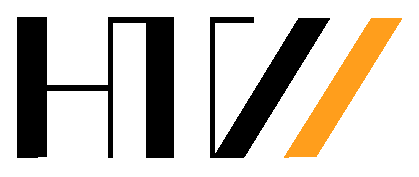
\includegraphics[height=1.7em]{../LaTeX_master/HTW-Logo.eps}}
	\ohead{\Dokumententitel}
	\ofoot{\footnotesize{\textcolor{darkgray}{Mitschrift von\\ \Dokumentenautor}}}
	% Titelseite
	\title{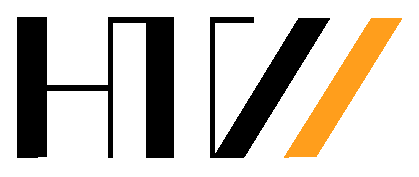
\includegraphics[width=0.35\textwidth]{../LaTeX_master/HTW-Logo.eps}\\\vspace{0.5em}
	\Huge\textbf{\Dokumententitel} \\\vspace*{0,5cm}
	\Large \Dokumentenuntertitel \\\vspace*{4cm}}
	\author{\textcolor{darkgray}{Mitschrift von \Dokumentenautor} \vspace*{1cm}\\\Dokumentennotiz}
}

%% EIGENE BEFEHLE

%Farbdefinitionen
\definecolor{red}{RGB}{180,0,0}
\definecolor{green}{RGB}{75,160,0}
\definecolor{blue}{RGB}{0,75,200}
\definecolor{orange}{RGB}{255,128,0}
\definecolor{yellow}{RGB}{255,245,0}
\definecolor{purple}{RGB}{75,0,160}
\definecolor{cyan}{RGB}{0,160,160}
\definecolor{brown}{RGB}{120,60,10}

% Textfarbe ändern
\newcommand{\tred}[1]{\textcolor{red}{#1}}
\newcommand{\tgreen}[1]{\textcolor{green}{#1}}
\newcommand{\tblue}[1]{\textcolor{blue}{#1}}
\newcommand{\torange}[1]{\textcolor{orange}{#1}}
\newcommand{\tyellow}[1]{\textcolor{yellow}{#1}}
\newcommand{\tpurple}[1]{\textcolor{purple}{#1}}
\newcommand{\tcyan}[1]{\textcolor{cyan}{#1}}
\newcommand{\tbrown}[1]{\textcolor{brown}{#1}}

% Umstellen der Tabellen Definition
\newcommand{\mpb}[1][.3]{\begin{minipage}{#1\textwidth}\vspace*{3pt}}
\newcommand{\mpe}{\vspace*{3pt}\end{minipage}}

\newcommand{\resultul}[1]{\underline{\underline{#1}}}
\newcommand{\parskp}{$ $\\}	% new line after paragraph
\newcommand{\corr}{\;\widehat{=}\;}
\newcommand{\mdeg}{^{\circ}}

\newcommand{\nok}[2]{\begin{pmatrix}#1\\#2\end{pmatrix}}	% n über k

% Definition von Titel, Autor usw.
\DTitel{Mathematik I}
\DUntertitel{Spicker}
\DAutor{Falk-Jonatan Strube}
\DNotiz{Vorlesung von Prof. Dr. Fabian Schwarzenberger}

\makeatletter
\renewcommand\tableofcontents{%
    \@starttoc{toc}%
}
\makeatother

\begin{document}

%\maketitle
%\newpage
\tableofcontents
\newpage

\chapter{Folgen und Reihen}
\section{Berechnen}
$\sum_0^n a \cdot q^n=a\cdot \frac{1-q^{n+1}}{1-q}$\\
oder $\sum_0^n a \cdot q^n=\frac{a}{1-q}$ für $|q|<1$ (bei $|q|>1$: divergent!)
Darauf achten:
\begin{itemize}
\item auf Untergrenze $0$ achten:\\
$\sum_1^5 a^n = \sum_0^5 a^n -1$ (Summe „erweitern“ und Erweitertes abziehen)\\
oder:\\
$\sum_1^5 a^n = \sum_0^4 a^{n+1}$ ($n$ entsprechend neuer Grenze anpassen)
\end{itemize}
\section{Rechenregeln}
\begin{itemize}
\item $\sum_{n=n_0}^\infty a_n$ und $\sum_{n=n_0}^\infty b_n$ konvergent mit Summe $a$ und $b$, dann gilt: 
\begin{itemize}
\item $\sum_{n=n_0}^\infty (a_n+b_n)= a + b$
\item $\sum_{n=n_0}^\infty c\cdot a_n= c\cdot a$
\end{itemize}
\item $\sum_{n=n_0}^\infty a_n$ absolut konvergent $\Leftrightarrow$ die Glieder $a_n$ lassen sich beliebig umordnen.
\item $\sum_{n=n_0}^\infty a_n$ und $\sum_{n=n_0}^\infty b_n$ absolut konvergent mit Summen $a$ und $b$, dann gilt:
\begin{itemize}
\item $\left(\sum_{i=0}^\infty a_i\right)\cdot \left( \sum_{j=0}^\infty b_j\right)=\sum_{i=0}^\infty  \sum_{j=0}^\infty a_i b_j=a\cdot b \qquad \left( =\sum_{n=0}^\infty  \sum_{i=0}^\infty a_i b_{n-i} \quad \text{Cauchy-Produkt}\right)$
\end{itemize}
\end{itemize}
\section{Konvergenz}
\begin{enumerate}
\item notwendige Bedingung:Eine Reihe kann nur konvergieren, wenn die entsprechende Folge eine $0$-Folge $\lim_{n\to\infty}a_n=0$ ist.
\item mit hinreichendem Kriterium prüfen:
\begin{itemize}
\item Vergleich:\\
Wenn $0\leq a_n\leq b_n$ und $\sum b_n$ konvergent, dann auch $\sum a_n$ konv. ($b_n$ ist konv. Majorante)\\
Wenn $0\leq b_n \leq a_n$ und $\sum b_n$ divergent, dann auch $\sum a_n$ div. ($b_n$ ist div. Minorante)\\
Vergleichsreihen: \\
$\sum_{n=1}^{\infty} \frac{1}{n^\lambda}=\begin{cases}
\text{konvergent} & \text{für }\lambda >1 \\
\text{divergent} & \text{für }\lambda \leq 1 
\end{cases}$\\
weitere siehe S. 74, S.77 Merziger
\item Quotientenkriterium\\
$\lim_{n\to \infty} \left| \frac{a_{n+1}}{a_n}\right|\begin{cases}
<1 & \sum_{n=n_0}^\infty \text{ absolut konvergent}\\
>1 & \sum_{n=n_0}^\infty \text{ divergent}\\
=1 & \text{keine Aussage}
\end{cases}$
\item Wurzelkriterium\\
$\lim_{n\to \infty} \sqrt[n]{|a_n|} \begin{cases}
<1 & \sum_{n=n_0}^\infty \text{ absolut konvergent}\\
>1 & \sum_{n=n_0}^\infty \text{ divergent}\\
=1 & \text{keine Aussage}
\end{cases}$
\item Leibnitz\\
Eine alternierende Reihe ist konvergent, wenn der Betrag der Folge eine $0$-Folge ist.
\end{itemize}
\end{enumerate} 

\section{Potenzreihen}
$\sum_{n=0}^\infty a_n (x-x_0)^n$: Potenzreihe mit Mittelpunkt $x_0$
\begin{itemize}
\item Wenn $r:=\lim_{n\to \infty} \left| \frac{a_n}{a_{n+1}}\right|=\lim_{n\to \infty} \frac{1}{\sqrt[n]{|a_n|}}$ existiert, dann:\\
$\sum_{n=0}^\infty a_n (x-x_0)^n\begin{cases}
\text{absolut konvergent} & \text{für }x\in \mathbb{R} \text{ mit }|x-x_0|<r\\
\text{divergent} & \text{für }x\in \mathbb{R} \text{ mit }|x-x_0|>r
\end{cases}$.\\
$r$: Konvergenzintervall um $x_0$ (darf auch $1$ sein)
\item Intervall: $(x_0-r, x_0+r)$ (wenn $r=0$, dann $\emptyset$)
\item Konvergenzbereich: $[x_0-r,x_0+r)$ ($[,],(,)$ je nach dem, ob Randpunkt konvergiert. Wenn $r=0$, dann $[r]$)\\
Wenn $r=\infty$: beständige Konvergenz
\item Radius im Abhängigkeit von $a_n$: Wenn $a_n\leq f(n)$, dann $r\geq \lim \dots$.
\end{itemize}
Wichtige Reihen:\\
$\sum_{n=0}^\infty x^n = \frac{1}{1-x}$ für $x\in (-1,1)$ (geometrische Reihe)\\
$\sum_{n=0}^\infty \frac{x^n}{n!}=e^x$ für $x\in \mathbb{R}$\\
weitere siehe Merziger F3

\chapter{Grenzwerte}
wichtige Grenzwerte:\\
$\lim_{x\to0}\frac{\sin (x)}{x}=1$\\ 
$\lim_{x\to 0} \frac{\sin (ax)}{x}=a$\\
$\lim_{x\to 0} \sin \frac{1}{x}$ existiert nicht.\\
weitere siehe Merziger F3
\begin{itemize}
\item Rechtsseitiger Grenzwert: $\lim_{x\searrow x_0}$
\item Linksseitiger Grenzwert: $\lim_{x\nearrow x_0}$
\end{itemize}
\begin{itemize}
\item Substituieren:\\
wenn bspw. Term in $\sin$ o.ä.
\item Term erweitern zum vereinfachen (bspw. binom. Formel): $a\cdot \frac{b}{b}$
\item l'Hopital: $\lim_{x\to a} \frac{f(x)}{g(x)}=\lim_{x \to a} \frac{f'(x)}{g'(x)}$ für $\frac{0}{0}$ oder $\frac{\infty}{\infty}$ (siehe Merziger S. 93)\\
Achtung: Wenn l'Hopital keine Lösung liefert: bspw. in Ursprungsgleichung etwas ausklammern.\\
Umformung von Gleichungen um l'Hopital anwenden zu können:\\
$f\cdot g = \frac{f}{\frac{1}{g}}$ (oder umgekehrt)\\
$f-g=f\left(1-\frac{g}{f}\right)$\\
$f^g=\exp(g\cdot \ln f)$
\end{itemize}
\section{Stetig}
Funktion ist stetig, wenn links- und rechtsseitiger Grenzwert gleich mit dem Grenzwert an dem Punkt.
\begin{itemize}
\item hebbar Stetig: wenn Grenzwert im Punkt nicht existiert, aber links- und rechtsseitiger Grenzwert gleich (bsp.: $\frac{\sin x}{x}$ an Stelle $0$) sind.
\item endlicher Sprung: wenn links- und rechtsseitiger Grenzwert nicht gleich sind, Grenzwert an der Stelle aber existiert.
\end{itemize}

\chapter{Differentiation}

\section{Regeln}
\begin{itemize}
\item $(A\,f+B\,f)' = A\,f'+B\,f'$
\item $(f\cdot g)' = f'g+fg'$
\item $\left(\frac{f}{g}\right)'=\frac{f'g+fg'}{g^2}$
\item $(f(g))'=f'(g)\cdot g'$
\item $(f^g)'=f^g\cdot \left(g'\cdot \ln f + g\frac{f'}{f}\right)$
\end{itemize}

\section{Taylor}
An der Stelle $x_0$ bis zum $n$-ten Grad:\\
$P_n(x)=f+\frac{f'}{1!}(x-x_0)+\frac{f''}{2!}(x-x_0)^2+\dots + \frac{f^{(n)}}{n!}(x-x_0)^n$\\
$R_n=f-P_n=\frac{f^{(n+1)}(\xi)}{(n+1)!}(x-x_0)^{n+1} \qquad \xi=x_0+\vartheta(x-x_0)\quad \vartheta \in (0,1)$

\paragraph{Fehler-Näherung} am Punkt $x_1$ mittels Restglied:\\
Maximale Abweichungen:
\begin{itemize}
\item $R_{n1}\frac{f^{(n+1)}(x_0)}{(n+1)!}(x_1-x_0)^{n+1}$
\item $R_{n2}\frac{f^{(n+1)}(x_1)}{(n+1)!}(x_1-x_0)^{n+1}$
\end{itemize}
Wert liegt damit zwischen $P_n+R_{n1}$ und $P_n+R_{n2}$.
\paragraph{Abweichung} und relativer Fehler:\\
absoluter Fehler (Ungenauigkeit): $P_n-f(x_0)$
relativer Fehler: $\frac{P_n-f(x_0)}{f(x_0)}$

\subsection{Taylor-Reihe}
$f(x)=\sum_{k=0}^\infty \frac{f^{(k)}(x_0)}{k!}(x-x_0)^k$ wenn $f$ beliebig oft diffbar und $R_n=0$

\section{Kurvendiskussion}
\begin{itemize}
\item Nullstellen\\
$n$-ter Ordnung: $f(x_0) = f'(x_0)=...=f^{(n-1)}(x_0)=0 \wedge f^n (x_0) \not = 0$
\item Extremstellen $f'(x_0)=0$\\
Hinreichend: \\
mit $n$ gerade ($f''$, …): $f^{(n)}\begin{cases}
<0 & \text{Maximum}\\
>0 & \text{Minimum}
\end{cases}$\\
(Wenn zusätzlich $f'=0$, dann Flachstelle)\\
oder: Wenn $f'(x_0)$ Vorzeichen wechselt: $\begin{cases}
\text{von }+ \text{ auf }-&\text{lokales Maximum}\\
\text{von }- \text{ auf }+&\text{lokales Minimum}\\
\text{kein VZW} & \text{Horizontal-Wendestelle}
\end{cases}$
\item Wendestellen $f'=f''=0$ (konvex/konkav von oben betrachtet)\\
mit $n$ ungerade ($f'''$, …): $f^{(n)}\begin{cases}
<0 & \text{konvex}\to \text{konkav}\\
>0 & \text{konkav}\to \text{konvex}
\end{cases}$\\
oder: Wenn $f''$ Vorzeichen wechselt: $\begin{cases}
\text{von }+ \text{ auf }-&\text{konvex}\to \text{konkav}\\
\text{von }- \text{ auf }+&\text{konkav}\to \text{konvex}\\
\text{kein VZW} & \text{Flachstelle}
\end{cases}$
\end{itemize}

\section{Kurvendarstellung}
\begin{itemize}
\item Parameter in explizite Darstellung:\\
Parameter $t$ eliminieren (Gleichungen miteinander verrechnen: $x+y=x(t)+y(t)$ [wenn sich damit das $t$ weg hebt] oder eine Gleichung nach $t$ auflösen und in die andere einsetzen: $y=y(t(x))$)
\item Explizite in Polardarstellung:\\
$x=r\cos\varphi$\\
$y=r\sin \varphi$
\item Explizite in Parameterdarstellung:\\
$x=t$, dann ist $y=y(t)$
\item Polar in Parameterdarstellung:\\
$x=r(\varphi)\cos\varphi$\\
$y=r(\varphi) \sin \varphi$
\end{itemize}

\subsection{Tangenten + Normalen}
Tangentengleichungen:\\
$y=y_0+m(x-x_0)$\\
$\vec{r}=\mtr{x\\y}=\mtr{x_0\\y_0}+s \cdot \vec{t} \quad s\in \mathbb{R}$\\
Normalengleichungen:\\
$y=y_0-\frac{1}{m}(x-x_0)$\\
$\vec{r}=\mtr{x\\y}=\mtr{x_0\\y_0}+s\cdot \vec{n} \quad s \in \mathbb{R}$\\
Allgemein: $m_n=-\frac{1}{m_t}$\\
\begin{tabular}{L{.18} | l | L{.18} | l}
Kurve & $y=f(x),\;x\in I$ & $x=x(t)$\newline $y=y(t), \; t\in I$ & $r(\varphi), \; \varphi \in I$ \\
\hline 
Punkt \newline$P_0=(x_0,y_0)$ & $P_0=(x_0,f(x_0))$ & $P_0=(x(t_0),y(t_0))$& $P_0=(r(\varphi_0)\cdot \cos\varphi_0 , \; r(\varphi_0) \cdot \sin \varphi_0$\\
Anstieg $m=\tan\alpha$ in $P_0$ & $f'(x_0)$ & $\frac{\dot{y}(t_0)}{\dot{x}(t_0)}$ & $\frac{r'(\varphi_0)\sin\varphi_0 + r(\varphi_0)\cos \varphi_0}{r'(\varphi_0)\cos\varphi_0 - r(\varphi_0)\sin \varphi_0}$\\
Tangenten-\newline vektor $\vec{t}$ & $\mtr{1\\ f'(x_0)}$ & $\mtr{\dot{x}(t_0) \\ \dot{y}(t_0)}$ & $\mtr{r'(\varphi_0)\cos\varphi_0 - r(\varphi_0)\sin \varphi_0\\r'(\varphi_0)\sin\varphi_0 + r(\varphi_0)\cos \varphi_0}$\\
Normalen-\newline vektor $\vec{n}$ & $\mtr{-f'(x_0) \\ 1}$ & $\mtr{-\dot{y}(t_0)\\\dot{x}(t_0)}$ & $\mtr{-r'(\varphi_0)\sin\varphi_0 - r(\varphi_0)\cos \varphi_0\\ r'(\varphi_0)\cos\varphi_0 - r(\varphi_0)\sin \varphi_0}$ \\
\end{tabular}\\

\subsection{Krümmung}
$K$… Krümmungskreis (Schmiegkreis)\\
$\varkappa$ (Kappa)… Krümmung\\
$\varrho$… Krümmungsradius mit $\varrho=\frac{1}{|\varkappa|}$\\
$M$… Mittelpunkt des Krümmungskreises $\overrightarrow{OM}=\mtr{x_0 \\ y_0}+\frac{1}{\varkappa}\cdot \frac{\vec{n}}{|\vec{n}|}$\\
\begin{tabular}{L{.2} | L{.3} | L{.199} | L{.3}}
Kurve & $y=f(x),\;x\in I$ & $x=x(t)$\newline $y=y(t), \; t\in I$ & $r(\varphi), \; \varphi \in I$ \\
\hline 
Krümmung $\varkappa$ in Punkt $P=(x,y)$ & $\varkappa=\frac{y''}{(1+(y')^2)^{\tfrac{3}{2}}}$ & $\varkappa=\frac{\dot{x}\ddot{y}-\ddot{x}\dot{y}}{(\dot{x}^2+\dot{y}^2)^{\tfrac{3}{2}}}$ & $\varkappa=\frac{r^2+2(r')^2-r\cdot r''}{(r^2+(r')^2)^{\tfrac{3}{2}}}$
\end{tabular}

\subsection{Tangente+Krümmung im Raum}
$\vec{r}=\vec{r}(t)=\mtr{x(t)\\y(t)\\z(t)}, \; t \in I, \; \vec{r}=\mtr{x\\ y \\ z}$\\
Tangente in $t_0$:\\
$\vec{g}(s)=\vec{r}(t_0)=\mtr{x(t_0)\\y(t_0)\\z(t_0)}+s\cdot \mtr{\dot{x}(t_0)\\\dot{y}(t_0)\\\dot{z}(t_0)}, \; s \in \RR$\\
Krümmung:\\
$\varkappa = \frac{|\dot{r}\times \ddot{r}|}{|\dot{r}|^3}$ (Ableitung Vektor: jede „Zeile“ ableiten)

\subsection{Newton zur Nullstellenbestimmung}
Rekursiv berechnet:\\
$x_{n+1}=x_n-\frac{f(n)}{f'(n)}$\\
\begin{tabular}{l | l}
$n$ & $x_n$\\
\hline 
$0$ & Startwert (Abschätzung, wo NS liegen könnte)\\
$1$ & $x_0-\frac{f(x_0)}{f'(x_0)}$\\
$2$ & $x_1-\frac{f(x_1)}{f'(x_1)}$
\end{tabular}

\chapter{Integration}
\begin{itemize}
\item Substitution:\\
Substituiere im Integral $\int f(g)\cdot g' \intd{x}$  $u=g$, dann ist $\diffd{x}=\frac{1}{g'}\diffd{u}$. Damit kürzt sich $g'$ weg und das Integral kann gelöst werden. Am Schluss Rücksubstituieren.\\
Bei bestimmten Integralen:\\
Entweder Grenzen ersetzen (Grenzen in $u$ einsetzen) oder Grenzen erst nach lösen und Rücksubstituieren auf Stammfunktion anwenden.
\item lineare Substitution:\\
$\int f(ax+b)\intd{x}$, substituiere $u=ax+b$ und damit $\diffd{x}=\frac{1}{a}\diffd{u}$
\item partielle Integration:\\
$\int f g' \intd{x}=fg-\int f' g \intd{x}$\\
Dann optimal, wenn $f'$ nicht mehr von $x$ abhängig ist oder sich mit $g$ wegkürzt ($\to f=\ln x$).\\
Dann entweder Integral berechenbar, oder wenn $f'g = fg'$: $\int fg'=\frac{1}{2}fg$.
\end{itemize}
\section{Partialbruchzerlegung}
Zum lösen von Integralen mit Brüchen
\begin{itemize}
\item Bruch muss unecht gebrochen sein. Wenn nicht ggf. mit Polynomdivision aufteilen: $a+\frac{r}{q}$ (Polynom+echt gebrochener Term)\\
Polynomdivision (Erinnerung):\\
$(x^3+2x^2+1)\div (x+1)=x^2+x-1+\frac{2}{x+1}$\\
$-(x^3+x^2)$\\
$\vdots$
\item Nullstellen des Nenners bestimmen und getrennt aufschreiben (ggf. reell und komplex): \\
$(x-x_{01})^n(x-x_{02})^n\cdots (x^2+p_1x+q_1)^m \cdots$ (Nullstellen jeweils mit Mehrfachheit $n$, bzw. $m$)
\item PBZ:\\
$\begin{cases}
(x-\alpha)^k\\
(x^2+px+q)^m
\end{cases}$ entspricht jeweils
$\begin{cases}
\frac{A_1}{x-\alpha}+\frac{A_2}{(x-\alpha)^2}+\dots + \frac{A_2}{(x-\alpha)^k}\\
\frac{B_1x+C_1}{x^2+px+q}+\frac{B_2 x + C_2}{(x^2+px+q)^2}+\dots + \frac{B_m x + C_m}{(x^2+px+q)^m}
\end{cases}$\\
Bsp.: $f(x) = \frac{x^2+4}{(x-1)^3(x+5)(x^2+2x+2)^2}\\
=\frac{A}{x-1}+\frac{B}{(x-1)^2}+\frac{C}{(x-1)^3}+ \frac{D}{x+5}+ \frac{Ex+F}{x^2+2x+2}+\frac{Gx+H}{(x^2+2x+2)^2}$
\item Ermittlung der Koeffizienten entweder durch Multiplikation mit Nenner vom Ansatz. Lösen durch wahlweise:
\begin{itemize}
\item Einsetzen der reellen Nullstellen
\item Koeffizientenvergleich
\end{itemize}
\item Integration der Summanden
\end{itemize}
\section{Numerische Integration}
Simpson:\\
$I \approx S_n(h)=\frac{h}{3}\left(\,(y_0+y_n)+4(y_1+y_3+\dots+y_{n-1})+2(y_2+y_4+\dots+y_{n-2})\,\right)$\\
Bsp.: $\int_0^1 e^{-x^2}\intd{x}$\\
$n=4, \; h=0,25$\\
\begin{tabular}{l l l l l}
$k$ & $x_k$ & $y_0, y_n$ & $y_{2j+1}$ & $y_{2j}$\\
\hline
0 & 0		& 1	&\\
1 & 0,25& 	&0,939413\\
2 & 0,5	&		&					& 0,778801\\
3 & 0,75&		&0,569783\\
4 & 1		& 0,367879\\
\hline 
 & &		1,367879 & 1,509196 & 0,778801
\end{tabular}\\
$S_4(0,25)=\frac{0,25}{3}\left(1,367879 + 4\cdot 1,509196 + 2\cdot 0,778801\right)$\\
$h=\frac{\text{obere Grenze}-\text{untere Grenze}}{n}$

\section{Uneigentliche Integral}
\subsection{Unendliches Intervall}
Uneigentliche Grenzen mit Parameter versehen und die berechnete Funktion mit $\lim$ lösen. Wenn beide Integralgrenzen uneigentlich sind, dann Integral aufteilen:\\
$\int_a^{\infty} f \intd{x} := \lim_{B \to \infty} \int_a^{B} f \intd{x}$\\
$\int_{-\infty}^{\infty} f \intd{x} := \int_{-\infty}^c f \intd{x} + \int_c^{\infty} f \intd{x}$ ($c$ beliebig, bspw. $c=0$).
\subsection{Unbeschränkter Integrand}
$\int_a^b f(x) \intd{x} := \lim_{\varepsilon \searrow 0} \int_a^{b-\varepsilon} f(x) \intd{x}$\\
falls Unendlichkeitsstelle $x_0$ im Inneren von $[a,b]$ liegt:\\
$\int_a^b f(x) \intd{x} := \int_a^{x_0} f(x) \intd{x} + \int_{x_0}^b f(x) \intd{x} \Rightarrow \lim_{\varepsilon\searrow 0} \int_a^{x_0-\varepsilon} f(x) \intd{x} + \lim_{\varepsilon\searrow 0} \int_{x_0 + \varepsilon}^b f(x) \intd{x}$\\
Bsp.: $\int_0^4 \frac{1}{\sqrt{x}}\intd{x} = \lim_{\varepsilon\searrow0} \left[2\sqrt{x}\right]_{\varepsilon}^4 = \lim_{\varepsilon \searrow 0} \left( 2 \sqrt{4}-2 \sqrt{\varepsilon}\right) = 4$
\section{Anwendungen}
\subsection{Flächeninhalte}
mit $a<b$ und $f(x) \geq 0$:\\
$F=\int_a^b f(x) \intd{x}$\\
mit $a<b<c$:\\
$F=\int_a^c |f(x)| \intd{x}=\left| \int_a^b f(x) \intd{x}\right| + \left| \int_b^c f(x) \intd{x}\right|= \int_a^b f(x) \intd{x} + \int_c^b f(x) \intd{x}$\\
mit $f(x)$: obere Funktion und $g(x)$: untere Funktion:\\
$F=\int_{x_1}^{x_2} f(x) - g(x) \intd{x}$
\subsection{Bogenlänge}
\begin{tabular}{l | l}
Kurvendarstellung & Bogenlänge $s$, Bogenelement $\diffd{s}$\\ 
\hline
$x=x(t),\; y=y(t),\; t \in [\alpha,\beta]$ & $s= \int_{\alpha}^{\beta} \underbrace{\sqrt{(\dot{x}(t))^2+(\dot{y}(t))^2}\intd{t}}_{\diffd{s}}$\\
$y =f(x),\; x\in [a,b]$ & $s=\int_a^b\underbrace{\sqrt{1+(f'(x))^2}\intd{x}}_{\diffd{s}}$\\
$x= g(y), \; y \in [c,d] $ & $s=\int_c^d\underbrace{\sqrt{1+(g'(y))^2}\intd{y}}_{\diffd{s}}$\\
$r=r(\varphi), \; \varphi\in [\alpha, \beta]$ & $s=\int_{\alpha}^{\beta}\underbrace{\sqrt{(r(\varphi))^2+(r'(\varphi))^2}\intd{\varphi}}_{\diffd{s}}$
\end{tabular}\\
Raumkurven:\\
$s=\int_{\alpha}^{\beta} \sqrt{(\dot{x}(t))^2+(\dot{y}(t))^2+(\dot{z}(t))^2}\intd{t}$
\subsection{Rotationsvolumen}
$V_x = \pi \cdot \int_a^b(f(x))^2\intd{x}$\\
$V_x=\pi \int_{\alpha}^{\beta} (y(t))^2\cdot \underbrace{\dot{x}(t) \intd{t}}_{\diffd{x}}$
\subsection{Mantelflächen}
mit jeweils $\diffd{s}$ aus Tabelle Bogenlänge\\
$M_x=2\pi \int_a^b \intd{s}=2\pi \int_a^b f(x) \sqrt{1+(f'(x))^2}\intd{x}$ bzw.\\
$M_y=2\pi \int_c^d g(y) \sqrt{1+(g'(y))^2}\intd{y}$ bzw. bei Parameter:\\
$M_x=2\pi \int_K y\intd{s}=2\pi \int_K y \sqrt{(\dot{x})^2+(\dot{y}	)^2}\intd{t}$
\subsection{Fourier-Reihe}
$f_n(x):= \frac{a_0}{2}+\sum_{k=1}^n a_k \cos (k\omega x) + b_k \sin (k \omega x )$\\
$a_0 = \frac{2}{T}\int_0^T f(x) \intd{x},\\
a_k = \frac{2}{T}\int_0^T f(x) \cos (k \omega x) \intd{x}, \\
b_k = \frac{2}{T} \int_0^T f(x) \sin (k \omega x) \intd{x}$ \qquad ($k\in \NN$)\\
Ist $f$ symmetrisch gilt (vereinfachend):\\
\begin{tabular}{l | l l l }
$f$ gerade & $a_0 = \frac{4}{T}\int_0^{\frac{T}{2}}f(x) \intd{x}$, $ a_k = \frac{4}{T}\int_0^{\frac{T}{2}}f(x) \cos (k\omega x) \intd{x}$, $ b_k =0$\\
\hline
$f$ ungerade & $a_0=0$, $a_k = 0$, $b_k = \frac{4}{T}\int_0^{\frac{T}{2}}f(x) \sin (k\omega x) \intd{x}$
\end{tabular}  

\section{Mehrere Veränderliche}
\begin{tabular}{L{0.5} | L{0.4}}
Volumen $V$ unter $z=f(x,y)\geq 0$ über $B$ & $V=\iint_B f(x,y) \intd{b}$\\
\hline
Flächeninhalt $[B]$ von $B$ & $[B]=\iint_B 1 \intd{b} = \iint_b \intd{b}$\\
\hline
geometrischer Schwerpunkt $(x_s, y_s)$ von $B$ & $x_s=\frac{1}{[B]}\iint_B x \intd{b}, \; y_s=\frac{1}{[B]}\iint_B y \intd{b}$\\
\hline 
Integralmittelwert $m$ von $f$ auf $B$ & $m=\frac{1}{[B]}\iint f(x,y) \intd{b}$
\end{tabular}\\
$\diffd{b} = r\intd{r}\intd{\varphi}$ (Polar)

\subsection{Koordinatentransformation}
$I=\iint_B f(x,y) \intd{b}= \iint_{B'}f(x(u,v), y(u,v)) \left| \frac{\partial (x,y)}{\partial (u,v)}\right| \intd{u}\intd{v}$ \\
Beispiel Polarkoordinaten: $\frac{\partial (x,y)}{\partial (x,y)}=\dtr{x_r & x_\varphi \\ y_r & y_\varphi}=\dtr{\cos \varphi & - r \sin \varphi \\ \sin \varphi & r \cos \varphi} = r \cos ^2\varphi + r \sin^2 \varphi = r$

\subsection{Oberflächen}
\begin{tabular}{L{0.5} | L{0.4}}
Flächeninhalt $[F]$ von $F$ & $[F]=\iint_F \intd{F}$\\
\hline
geometrischer Schwerpunkt $(x_s,y_s,z_s)$ & $x_s = \frac{1}{[F]}\iint_F x \intd{F}$\\&$y_s = \frac{1}{[F]}\iint_F y \intd{F}$\\&$z_s=\frac{1}{[F]}\iint_F z \intd{F}$\\
\hline
Integralmittelwert $m$ von $f$ auf $F$ & $m=\frac{1}{[F]}\iint_F f(x,y,z) \intd{F}$
\end{tabular}\\
Berechnung von $\diffd{F}=|\vec{r}_u\times \vec{r}_v| \intd{u}\intd{v}$\\
\begin{tabular}{L{0.5} | L{0.4}}
Fläche & $\diffd{F}$\\
$z=f(x,y)$ … expl. karth. Darstellung & $\diffd{F}=\sqrt{1+f_x^2+f_y^2}\intd{x}\intd{y}$\\
$z=f(r,\varphi)$ … expl. zyl. Darstellung & $\diffd{F}=\sqrt{r^2(1+f_r^2)+f_\varphi^2}\intd{r}\intd{\varphi}$\\
Speziell für Rotationsflächen $z=f(r,\varphi)=g(r), \; \varphi \in [0,2\pi]$ & $\diffd{F}=r\sqrt{1+(g'(r))^2}\intd{r}\intd{\varphi}$\\
Kugel MP $0$, Radius $R$ & $\diffd{F}=R^2\sin \vartheta \intd{\varphi}\intd{\vartheta}$
\end{tabular}

\chapter{Differentialrechnung mehrerer Veränderlicher}
\begin{itemize}
\item Satz von Schwarz: $f_{xy}=f_{yx}$
\item Kettenregel: $z=f(g(x,y), h(x,y))$:\\
$z_x=z_u\cdot u_x + z_v \cdot v_x\\
z_y=z_u \cdot u_y + z_v \cdot v_y$\\
Bsp.: $z=(x^2+3y^2)^{x+2y}$ $\Rightarrow$ $u=x^2+3y^2, \; v=x+2y \;\Rightarrow\; z=f(u,v)=u^v$
\item $f'(x)=-\frac{F_x}{F_y}$ (implizite Funktion)\\
gilt, wenn $F=0$ und $F_y\not = 0$
\item Gradient $\nabla f$: Vektor, in dem jede Zeile nach der jeweiligen Variablen abgeleitet ist.
\end{itemize}

\section{Fehlerrechnung}
Gesamtfehler $S_f=|f_x(x_0,y_0,\dots)|\cdot S_x+|f_y(x_0,y_0,\dots)|\cdot S_y+\dots$ mit $S_y$ jeweils die Messfehler der einzelnen Variablen und $x_0$ die gemessen Fehler

\section{Richtungsableitung}
$\frac{\partial f}{\partial s} (x_0,y_0) = f_x(x_0,y_0) \cdot \cos \alpha + f_y (x_0,y_0) \cdot \sin \alpha$  (wenn Winkel gegeben)\\
$= \frac{f_x(x_0,y_0) \cdot s_1+f_y (x_0,y_0) \cdot s_2}{\sqrt{s_1^2+s_2^2}}$ (wenn $\vec{s}$ gegeben)

\subsection{Tangentialebene}
$\left(\mtr{F_x(x_0,y_0,z_0)\\F_y(\dots)\\F_z(\dots)}, \mtr{x-x_0\\y-y_0\\z-z_0}\right) = 0$

\section{Extrema}
\subsection{Ohne Nebenbedingung}
notwendige Bedingung $f_x'=0$ und $f_y'=0$\\
hinreichende Bedingung $f_{xx}f_{yy}-f_{xy}^2>0$: lokal extremal und mit $f_{xx}\begin{cases}
<0 & \text{lokal maximal}\\
>0 & \text{lokal minimal}
\end{cases}$
\subsection{Mit Nebenbedingung}
Lagrange-Funktion: $F(x,y,\lambda)=f+\lambda g$ mit $f$: Funktion und $g$: Nebenbedingung\\
Gleichungssytem $F_x=0$, $F_y=0$, $F_\lambda =0$ lösen. Ergebnis sind Extrema.\\
Untersuchung, ob Maximum oder Minimum per geometr. Überlegung.

\chapter{Differentialgleichungen}
\section{Mit trennbaren Variablen}
\begin{tabular}{L{0.49} L{0.49}}
Typ: $y'=f(x) \cdot g(y)$ & Bsp. 1: $y'=x\cdot y^2$, $y(1)=-2$\\
\hline
Lösungsmethode &\\
1. Gleichung aufstellen & \\
$\frac{\diffd{y}}{\diffd{x}}=f(x) \cdot g(y)$ & $\frac{\diffd{y}}{\diffd{x}}=x\cdot y^2$\\\hline
2. Trennung der Veränderlichen & \\
$\frac{\diffd{y}}{g(y)}= f(x) \intd{x}$ & $\frac{\diffd{y}}{y^2}= x \intd{x}$\\\hline
3. beide Seiten integrieren:&\\
$\int\frac{\diffd{y}}{g(y)}=\int f(x) \intd{x}$ & $\int\frac{\diffd{y}}{y^2}=\int x \intd{x}$\\
$G(y) = F(x)+C$ ($G(y)$: Stammfunktion von $\frac{1}{g(y)}$)& $-\frac{1}{y}=\frac{x^2}{2}+C$\\
(allgemeine Lösung, implizit)\\\hline
4. Falls möglich: Auflösen nach $y$&\\
$y=y(x)=\varphi(x,C)$ & $y=-\frac{1}{\frac{x^2}{2}+C}$\\
(allgemeine Lösung, explizit)\\\hline
5. Untersuchen von $g(y)=0$ (Nebenlösungen)&\\
& $y^2=0 \Leftrightarrow y=0$ (erfüllt ebenfalls die DGL: Nebenlösung)\\
6. Bei AWP: AB erfüllen & \\
& $x=1, \; y=-2$ einsetzen in DGL\\
& $\frac{1}{2}=\frac{1}{2}+C \Rightarrow C=0$\\
& Lösung des AWP: $y=-\frac{2}{x^2}$
\end{tabular}

\section{Lineare DGL 1. Ordnung}
Normalform: $y'+a(x)y=h(x)$
\begin{itemize}
\item Falls $h(x)=0$: homogen
\item Falls $h(x) \not = 0$: inhomogen
\end{itemize}
Lösung:
\begin{itemize}
\item $y_h$ homogene Lösung mit $h(x)=0$ (also trennbare Variablen) hat Art $y_h=C\cdot \dots$
\item $y_p$ partikuläre Lösung. Ansatz $y_p=C(x)\cdot a(x)$, damit $y'$ berechnen und in Ursprungsgleichung einsetzen. Damit wird $C(x)$ berechnet, was dann wieder in $y_p$ eingesetzt werden kann und zum Ergebnis führt.
\item $y=y_h+y_p$
\end{itemize}

\section{Ähnlichkeits-DGL}
\begin{anumerate}
\item Typ $\boxed{y'=f\left(\frac{y}{x}\right)}$\\
Lösung: Substitution $\frac{y}{x}=u=u(x)$, d.h. $y=u\cdot x$.\\
Also $y'=u'x+u$.\\
$\Rightarrow $ DGL mit trennbaren Variablen für $u=u(x)$\\
$\rightsquigarrow$ Lösen $\rightsquigarrow$ Rücksubstitution
\item Typ $\boxed{y'=y(ax+by+c)}$\\
Lösung: Substitution $ax+by+c=u(x)$, d.h. $u'=a+by'$.\\
Also $y'=\frac{1}{b}(u'-a)$.\\
Dann weiteres vorgehen wie bei a.)
\end{anumerate}










\end{document}